\documentclass[12pt, a4paper]{article}

\usepackage[hmargin=2.5cm, vmargin=2cm]{geometry}
\usepackage{amsthm, amssymb, mathtools, yhmath, graphicx}
\usepackage{fontspec, type1cm, titlesec, titling, fancyhdr, tabularx}
\usepackage{color}
\usepackage{unicode-math}
\usepackage{float}
\usepackage{subfig}
\usepackage{hhline}
\usepackage{comment}
\usepackage{siunitx}
\usepackage{csvsimple}
\usepackage{subcaption}

\usepackage[CheckSingle, CJKmath]{xeCJK}
\usepackage{CJKulem}
\usepackage{enumitem}
\usepackage{tikz}
\usepackage[siunitx]{circuitikz}
\usepackage{wrapfig}
%\setCJKmainfont[BoldFont=cwTex Q Hei]{cwTex Q Ming}
%\setCJKsansfont[BoldFont=cwTex Q Hei]{cwTex Q Ming}
%\setCJKmonofont[BoldFont=cwTex Q Hei]{cwTex Q Ming}
\setCJKmainfont[BoldFont=cwTeX Q Hei]{cwTeX Q Ming}

\def\normalsize{\fontsize{12}{18}\selectfont}
\def\large{\fontsize{14}{21}\selectfont}
\def\Large{\fontsize{16}{24}\selectfont}
\def\LARGE{\fontsize{18}{27}\selectfont}
\def\huge{\fontsize{20}{30}\selectfont}

%\titleformat{\section}{\bf\Large}{\arabic{section}}{24pt}{}
%\titleformat{\subsection}{\large}{\arabic{subsection}.}{12pt}{}
%\titlespacing*{\subsection}{0pt}{0pt}{1.5ex}

\parindent=24pt

\DeclarePairedDelimiter{\abs}{\lvert}{\rvert}
\DeclarePairedDelimiter{\norm}{\lVert}{\rVert}
\DeclarePairedDelimiter{\inpd}{\langle}{\rangle}
\DeclarePairedDelimiter{\ceil}{\lceil}{\rceil}
\DeclarePairedDelimiter{\floor}{\lfloor}{\rfloor}

\newcommand{\unit}[1]{\:(\text{#1})}
\newcommand{\df}[1]{\mathop{}\!\mathrm{d^#1}}
\newcommand{\img}{\mathrm{i}}
\newcommand{\dD}{\mathrm{d}}
\newcommand{\dI}{\,\mathrm{d}}

\title{ \bf {\Huge 電子電路實驗2: Active Filters}\\ 實驗結報}
\author{B02901178 江誠敏}

\begin{document}

\maketitle


\section{實驗結果}
\begin{center}
  \begin{tabular}{p{3cm}p{3cm}p{3cm}p{3cm}}
	\hline
  頻率 & $A_{bp}$ & $A_{hp}$ & $A_{lp}$\\
	\hhline{====}
  \SI{100}\Hz & 0.093 & 1.030 & 0.106\\
\SI{1}\kHz & 0.750 & 1.040 & 0.152\\
\SI{10}\kHz & 0.869 & 1.160 & 0.374\\
\SI{50}\kHz & 0.432 & 0.200 & 1.062\\
\SI{100}\Hz & 0.232 & 0.104 & 1.082\\
\SI{200}\Hz & 0.158 & 0.075 & 0.915\\

	\hline
\end{tabular}
\end{center}
\begin{figure}[H]
\begin{center}
  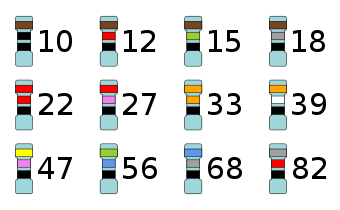
\includegraphics[width=0.75\textwidth]{fig1.pdf}
\end{center}
\caption{Bode plot}
\label{fig:}
\end{figure}
\section{結報問題}

\begin{enumerate}[itemsep=20pt, topsep=10pt]

  \item {In this experiment, the active filters were designed to pass through the 3dB frequency with the decay slope of 40dB/decade. Is that possible to be done by the slope of 20dB/decade? If it is so, try to explain the advantages or disadvantages of these two types of implementations.} \\[10pt]
    答:\\
    接一個普通的一階 filter 就可以讓 $f_{3db}$ 在 \SI{20}{\dB\per decade}。
    好處是只需要一顆 OP AMP ,比較省電。 壞處是斜率較平緩,可能濾的比較不乾淨。
      

  \item {For the measured data, analyze whether the theoretical values differ from experimental ones. Explain the reasons if they are not identical. Additionally, express how to improve the imperfection.} \\[10pt]
    答:\\
    以下是理論上的 Bode plot:
    \begin{figure}[H]
      \begin{center}
        \includegraphics[width=0.75\textwidth]{fig2.pdf}
      \end{center}
      \caption{Theoretically plot}
      \label{fig:}
    \end{figure}
    與實驗結果大致相同,但還是有一點差別。 \\
    以下列出造成差別的可能原因以及改進的方法:
    \begin{enumerate}
      \itemsep=0pt
      \item $\mu$a741 自身的頻率響應: 可能需要重新設計電路,比如利用負回饋電路的方法降低
        此效應。
      \item 實驗中元件的誤差: 可以在接電路前先量測、檢查電路元件的準確度。
      \item 量測的誤差: 多量幾次,確定量測方法的正確性。
    \end{enumerate}


  \item {Is it possible to implement a band-pass filter by applying the circuit in Fig. 2 and Fig. 3? Why? Use PSPICE simulations to describe your designed circuit diagrams.} \\[10pt]
    答:
    可以,把 SAB High pass filter 的輸出端接到 SAB Low pass filter 的輸入端,
    SAB low pass filter 的輸出即等同一個 Band pass filter 的輸出.

    Ngspice 的模擬圖:
    \begin{figure}[H]
      \begin{center}
        \includegraphics[width=0.75\textwidth]{fig3.pdf}
      \end{center}
      \caption{Ngspice simulation}
      \label{fig:}
    \end{figure}

  \item {4. Continuing the problem 3, compare the band-pass filter in Fig. 1
    and the one in problem 3, which one is better for? Why? } \\[10pt]
    答:
    可能各有優缺點。 在 Fig. 1 的 TIL filter 的優點是多工能性 (同時可以有低、
    高和帶通) , 且受元件的誤差影響較小。 而 Problem 3 中兩個 SAB filter
    串起的 filter 使用的 Op AMP 少一個,會較省電。


\end{enumerate}

\section{心得}
新學期開始了,又要開始做電電實驗了。 好在第一次的電電實驗比較簡單,
一下子就做完了。 不過後來才知道原來這一次的實驗其實是運氣 game ,
就看到做我對面的人運氣有夠差,弄了半天弄不出來,才發現
3 個 $\mu$a741 壞了 2 個 , 拿去換新的回來做,還是不行,原來是
新拿來的兩個之中又壞了一個,看他們做的一把鼻涕一把眼淚,下次做實驗還
是先去拜拜好了。
\end{document}

